\documentclass{beamer}
\usetheme{default}
\usepackage{url}
\usepackage{listings}
\usepackage{tikz}
\usetikzlibrary{arrows}

\title{Implicit surface geometry in Python with xyzcad}
\author{Stefan Helmert}
\begin{document}
	\begin{frame}[plain]
		\maketitle
	\end{frame}
	\begin{frame}{What is this?}
		\begin{tabular}{ccc}
			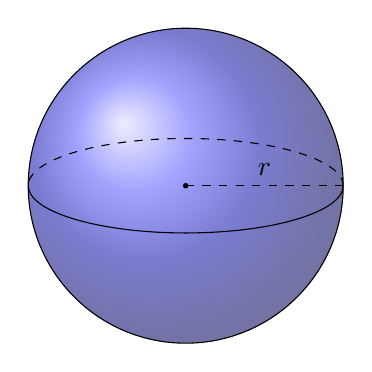
\begin{tikzpicture}
				\shade[ball color = blue!80, opacity = 0.6] (0,0) circle (2cm);
				\draw (0,0) circle (2cm);
				\draw (-2,0) arc (180:360:2 and 0.6);
				\draw[dashed] (2,0) arc (0:180:2 and 0.6);
				\fill[fill=black] (0,0) circle (1pt);
				\draw[dashed] (0,0 ) -- node[above]{$r$} (2,0);
			\end{tikzpicture}
			& \hspace{1cm} &
			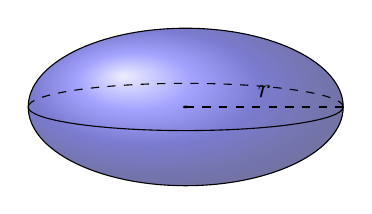
\begin{tikzpicture}[yscale=0.5]
				\shade[ball color = blue!80, opacity = 0.6] (0,0) circle (2cm);
				\draw (0,0) circle (2cm);
				\draw (-2,0) arc (180:360:2 and 0.6);
				\draw[dashed] (2,0) arc (0:180:2 and 0.6);
				\fill[fill=black] (0,0) circle (1pt);
				\draw[dashed] (0,0 ) -- node[above]{$r$} (2,0);
			\end{tikzpicture}\\
			$r^2 = x^2 + y^2 + z^2$	&  & $r^2 = x^2 + y^2 + \left(2 \cdot z\right)^2$\\
		\end{tabular}
		\vspace{1cm}\\
		\url{https://en.wikipedia.org/wiki/Implicit_surface}
		\url{https://de.wikipedia.org/wiki/Implizite\_Fl\%C3\%A4che}
	\end{frame}
		\begin{frame}{3D printing}
		\centering
		\textbf{STL file needed!}\\
		\vspace{0.5cm}
					
		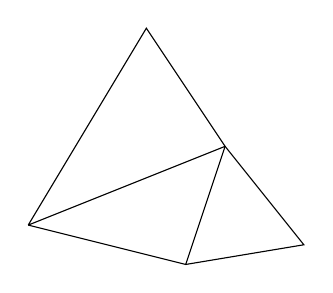
\begin{tikzpicture}[scale=0.5]
			\draw (0,0) -- (3,5) -- (5,2) -- (0,0);
			\draw (5,2) -- (4,-1) -- (0,0);
			\draw (5,2) -- (7,-0.5) -- (4,-1);
		\end{tikzpicture}\\
				\vspace{0.5cm}
		triangles to describe the surface of the volume
						\vspace{0.5cm}\\
		\url{https://en.wikipedia.org/wiki/STL_(file_format)}
		\url{https://de.wikipedia.org/wiki/STL-Schnittstelle}
	\end{frame}
	\begin{frame}{Material is True}
			\centering
		\begin{tabular}{ccc}
			\textbf{surface} & & \textbf{volume} \\			
			\begin{tikzpicture}
				\draw (0,0) circle (2cm);
			\end{tikzpicture}
			& \hspace{1cm} &
			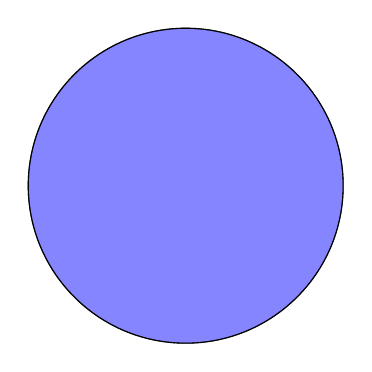
\begin{tikzpicture}
				\draw[fill = blue!80, opacity = 0.6] (0,0) circle (2cm);
				\draw (0,0) circle (2cm);
			\end{tikzpicture}\\
			$r^2 = x^2 + y^2 + z^2$	&  & $r^2 > x^2 + y^2 + z^2$\\
			equation & & inequality \\
		\end{tabular}
		\vspace{1cm}\\
		Inequalities are easier to handle!
	\end{frame}
	\begin{frame}{Find object}
		\centering
		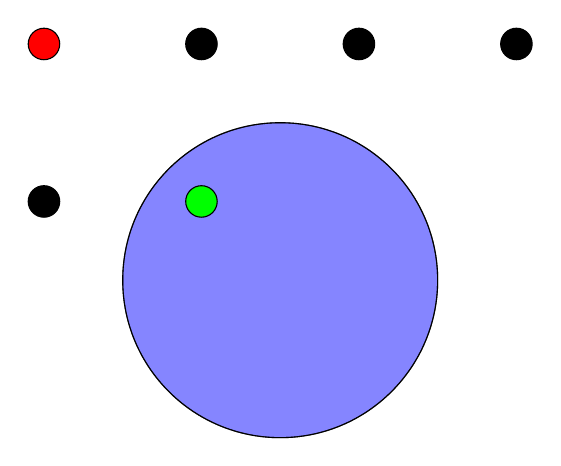
\begin{tikzpicture}			
			\draw[fill = blue!80, opacity = 0.6] (0,0) circle (2cm);
			\draw (0,0) circle (2cm);
			\draw[fill=red] (-3,3) circle (2 mm);
			\draw[fill=black] (-1,3) circle (2 mm);
			\draw[fill=black] (1,3) circle (2 mm);
			\draw[fill=black] (3,3) circle (2 mm);
			\draw[fill=black] (-3,1) circle (2 mm);
			\draw[fill=green] (-1,1) circle (2 mm);
		\end{tikzpicture}\\
	\end{frame}
	\begin{frame}{Find point on surface}
		\centering
		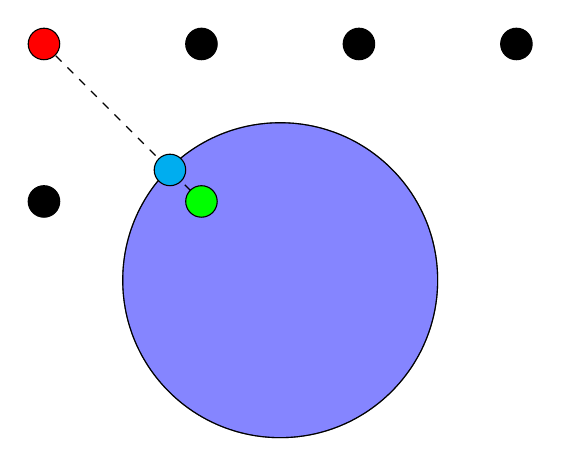
\begin{tikzpicture}			
			\draw[fill = blue!80, opacity = 0.6] (0,0) circle (2cm);
			\draw (0,0) circle (2cm);
			\draw[dashed] (-3,3) -- (-1,1);
			\draw[fill=red] (-3,3) circle (2 mm);
			\draw[fill=black] (-1,3) circle (2 mm);
			\draw[fill=black] (1,3) circle (2 mm);
			\draw[fill=black] (3,3) circle (2 mm);
			\draw[fill=black] (-3,1) circle (2 mm);
			\draw[fill=green] (-1,1) circle (2 mm);
			\draw[fill=cyan] (-1.4,1.4) circle (2 mm);
		\end{tikzpicture}\\
	\end{frame}
	\begin{frame}{Marching Cubes algorithm}
		\centering
		
		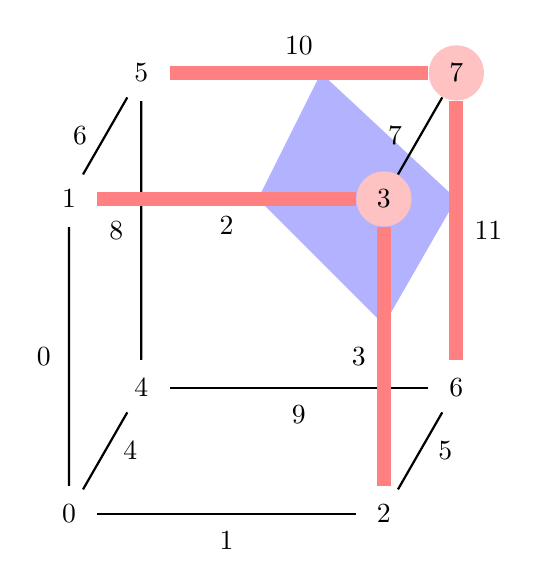
\begin{tikzpicture}[scale=4]
			\tikzstyle{vertex}=[circle,minimum size=20pt,inner sep=0pt]
			\tikzstyle{selected vertex} = [vertex, fill=red!24]
			\tikzstyle{selected edge} = [draw,line width=5pt,-,red!50]
			\tikzstyle{surface} = [fill=blue!30]
			\tikzstyle{edge} = [draw,thick,-,black]
			
			\path[surface] (0.8,1.4) -- (1.23,1) -- (1,0.6) -- (0.6,1) -- cycle;
			
			\node[vertex] (v0) at (0,0) {0};
			\node[vertex] (v1) at (0,1) {1};
			\node[vertex] (v2) at (1,0) {2};
			\node[selected vertex] (v3) at (1,1) {3};
			\node[vertex] (v4) at (0.23, 0.4) {4};
			\node[vertex] (v5) at (0.23,1.4) {5};
			\node[vertex] (v6) at (1.23,0.4) {6};
			\node[selected vertex] (v7) at (1.23,1.4) {7};
			
			\draw[edge] (v0) -- node[left=1mm] {0} (v1) -- node[below=1mm] (e2) {2} (v3) -- node[left=1mm] (e3) {3} (v2) --  node[below=1mm] {1} (v0);
			\draw[edge] (v0) -- node[right=1mm] {4} (v4) -- node[left=1mm] {8} (v5) -- node[left=1mm] {6} (v1) -- (v0);
			\draw[edge] (v2) -- node[right=1mm] {5} (v6) -- (v7) -- node[left=1mm] {7} (v3) -- (v2);
			\draw[edge] (v4) -- node[below=1mm] {9} (v6) --node[right=1mm] (e11) {11}  (v7) -- node[above=1mm] (e10) {10} (v5) -- (v4);
			
			\draw[selected edge] (v5) -- (v7);
			\draw[selected edge] (v3) -- (v1);
			\draw[selected edge] (v3) -- (v2);
			\draw[selected edge] (v6) -- (v7);
		\end{tikzpicture}

		\url{https://en.wikipedia.org/wiki/Marching_cubes}
		\url{https://de.wikipedia.org/wiki/Marching_Cubes}
	\end{frame}
	\begin{frame}{Higher precision}
		\centering
		
		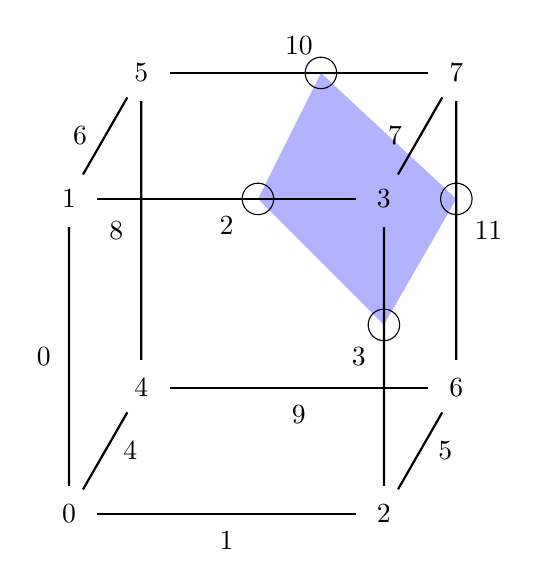
\begin{tikzpicture}[scale=4]
			\tikzstyle{vertex}=[circle,minimum size=20pt,inner sep=0pt]
			\tikzstyle{selected vertex} = [vertex, fill=red!24]
			\tikzstyle{selected edge} = [draw,line width=5pt,-,red!50]
			\tikzstyle{surface} = [fill=blue!30]
			\tikzstyle{edge} = [draw,thick,-,black]
			
			\path[surface] (0.8,1.4) -- (1.23,1) -- (1,0.6) -- (0.6,1) -- cycle;
			
			\node[vertex] (v0) at (0,0) {0};
			\node[vertex] (v1) at (0,1) {1};
			\node[vertex] (v2) at (1,0) {2};
			\node[ vertex] (v3) at (1,1) {3};
			\node[vertex] (v4) at (0.23, 0.4) {4};
			\node[vertex] (v5) at (0.23,1.4) {5};
			\node[vertex] (v6) at (1.23,0.4) {6};
			\node[ vertex] (v7) at (1.23,1.4) {7};
			
			\draw[edge] (v0) -- node[left=1mm] {0} (v1) -- node[below=1mm] (e2) {2} (v3) -- node[left=1mm] (e3) {3} (v2) --  node[below=1mm] {1} (v0);
			\draw[edge] (v0) -- node[right=1mm] {4} (v4) -- node[left=1mm] {8} (v5) -- node[left=1mm] {6} (v1) -- (v0);
			\draw[edge] (v2) -- node[right=1mm] {5} (v6) -- (v7) -- node[left=1mm] {7} (v3) -- (v2);
			\draw[edge] (v4) -- node[below=1mm] {9} (v6) --node[right=1mm] (e11) {11}  (v7) -- node[above=1mm] (e10) {10} (v5) -- (v4);
			
			\draw[ edge] (v5) -- (v7);
			\draw[ edge] (v3) -- (v1);
			\draw[ edge] (v3) -- (v2);
			\draw[ edge] (v6) -- (v7);
			
			\draw (0.8,1.4) circle (0.5 mm);
			\draw (1.23,1) circle (0.5 mm);
			\draw (1,0.6) circle (0.5 mm);
			\draw (0.6,1) circle (0.5 mm);
		\end{tikzpicture}
		
		Find exact position, where the surface separates cube edge.
	\end{frame}
	\begin{frame}{Triangles}
		\centering
		
		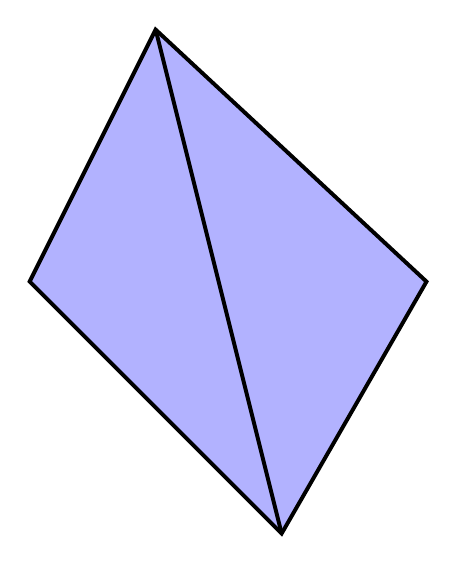
\begin{tikzpicture}[scale=8,line width=0.5mm]
			\tikzstyle{surface} = [fill=blue!30]
			\path[surface,draw] (0.8,1.4) -- (1.23,1) -- (1,0.6) -- (0.6,1) -- cycle;
			\draw (0.8,1.4) -- (1,0.6);
		\end{tikzpicture}
		
	\end{frame}
	\begin{frame}{Data flow}
		\centering
		
		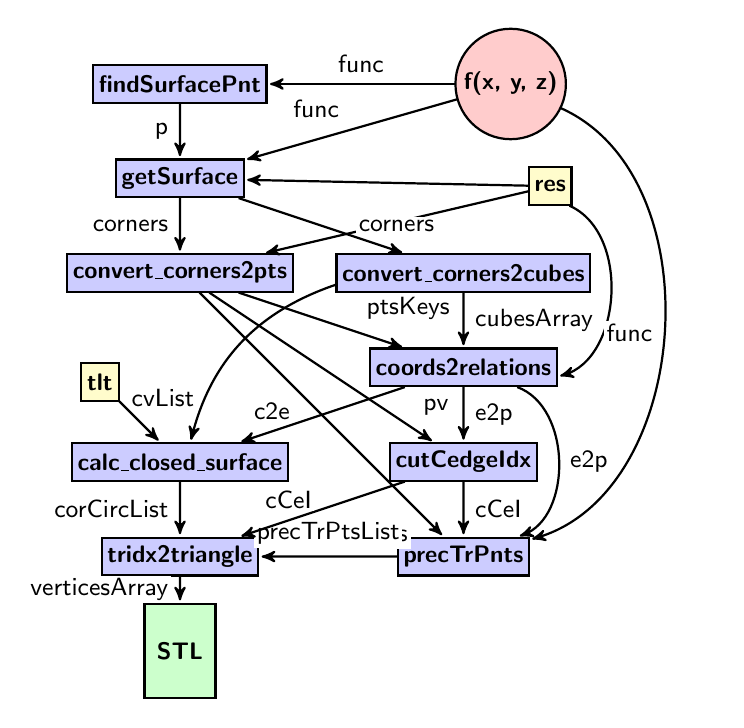
\begin{tikzpicture}[->,>=stealth',shorten >=1pt,auto,node distance=2cm,
			thick,main node/.style={rectangle,fill=blue!20,draw,
				font=\sffamily\Large\bfseries,minimum size=8mm},
			fun node/.style={circle,fill=red!20,draw,
				font=\sffamily\Large\bfseries,minimum size=8mm},
			file node/.style={rectangle,fill=green!20,draw,
				font=\sffamily\Large\bfseries,minimum height=20mm,minimum width=15mm},
			const node/.style={rectangle,fill=yellow!20,draw,
				font=\sffamily\Large\bfseries,minimum size=8mm},
				scale=0.6, every node/.append style={transform shape}
			]
			
			\node[main node] (SP) {findSurfacePnt};
			\node[fun node] (F) [right of=SP, node distance=7cm] {f(x, y, z)};
			\node[main node] (S) [below of=SP] {getSurface};
			\node[main node] (PTS) [below of=S] {convert\_corners2pts};
			\node[main node] (CBS) [right of=PTS, node distance=6cm] {convert\_corners2cubes};
			\node[main node] (R) [below of=CBS] {coords2relations};
			\node[main node] (CCI) [below of=R] {cutCedgeIdx};
			\node[main node] (PPTS) [below of=CCI] {precTrPnts};
			
			
			\node[main node] (CS) [left of=CCI, node distance=6cm] {calc\_closed\_surface};
			\node[const node] (TLT) [above left of=CS, node distance=2.4cm] {tlt};
			\node[const node] (RES) [above right of=CBS, node distance=2.6cm] {res};
			%	\node[main node] (TC) [below of=CS] {TrIdx2TrCoord};
			%	\node[main node] (CT) [below of=TC] {calcTrianglesCor};
			\node[main node] (TT) [below of=CS] {tridx2triangle};
			\node[file node] (STL) [below of=TT] {STL};
			
			\path[every node/.style={font=\sffamily\small,
				fill=white,inner sep=1pt}]
			(F) edge  node[above=1mm] {func} (SP)		
			(RES) edge (S)		
			(F) edge node[above left=1mm] {func} (S)		
			(SP) edge node[left=1mm] {p} (S)		
			%	() edge [bend left=30] node[left=1mm] {res} (S)	
			(RES) edge (PTS)			
			(S) edge node[left=1mm] {corners} (PTS)		
			%	() edge [bend left=30] node[left=1mm] {res} (PTS)		
			(S) edge node[above=2mm,pos=0.95] {corners} (CBS)	
			(RES) edge [bend left=70] (R)				
			(CBS) edge node[right=1mm] {cubesArray} (R)		
			(PTS) edge node[above right=1mm,pos=0.7] {ptsKeys} (R)		
			%	() edge [bend left=30] node[left=1mm] {res} (R)		
			(PTS) edge node[above right=1mm,pos=0.9] {pv} (CCI)		
			(R) edge node[right=1mm] {e2p} (CCI)		
			(F) edge [bend left=70] node[left=1mm] {func} (PPTS)		
			(CCI) edge node[right=1mm] {cCeI} (PPTS)		
			(R) edge [bend left=70] node[right=1mm] {e2p} (PPTS)		
			(PTS) edge node[below left=1mm,pos=0.9] {ptsKeys} (PPTS)		
			%	() edge [bend left=30] node[left=1mm] {tlt} (CS)		
			(TLT) edge  (CS)		
			(CBS) edge [bend right=10mm] node[left=1mm,pos=0.8] {cvList} (CS)		
			(R) edge node[above=1mm,pos=0.8] {c2e} (CS)		
			%	(PPTS) edge node[above=1mm] {precTrPtsList} (TC)		
			%	(CCI) edge node[above=1mm] {cCeI} (TC)		
			%	(CS) edge node[left=1mm] {corCircList} (TC)		
			(PPTS) edge node[above=1mm] {precTrPtsList} (TT)		
			(CCI) edge node[above=1mm,pos=0.7] {cCeI} (TT)		
			(CS) edge node[left=1mm] {corCircList} (TT)		
			%	(TC) edge  node[left=1mm] {circPtsCoordList} (CT)
			(TT) edge node[left=1mm] {verticesArray} (STL)		
			;
			
			
		\end{tikzpicture}
				
	\end{frame}
	\begin{frame}{Project}

		\textbf{Open Source}
		\vspace{0.3cm}
		
		\url{https://github.com/TheTesla/xyzcad}
		\vspace{1cm}

		\textbf{PyPI}
		\vspace{0.3cm}
		
		\texttt{pip install --upgrade xyzcad}

		\vspace{1cm}
		
		\textbf{Telegram Group}
		\vspace{0.3cm}
				
		\url{https://t.me/xyzcad_de_grp}
		
	\end{frame}
\end{document}
